\chapter{Using sitewise selective pressures to estimate the distribution of selective coefficients in mammals}
\label{ch_dfe}
\acresetall

\subsection{Modeling the global distribution of sitewise selective pressures}
\label{modeling_distr}

\begin{landscape}
\begin{table}
\centering \footnotesize
\begin{tabular}{lllrrrrrrrrrrrrrrr}
\toprule
 &  
 & \multicolumn{2}{c}{Log-normal} 
 & \multicolumn{2}{c}{Gamma} 
 & \multicolumn{2}{c}{Exponential} 
 & \multicolumn{2}{c}{Beta} 
 & \multicolumn{2}{c}{Weibull} \\
\cmidrule(r){3-4}
\cmidrule(r){5-6}
\cmidrule(r){7-8}
\cmidrule(r){9-10}
\cmidrule(r){11-12}

Species Set & Data Type
 & \omgmean & \% $>1$
 & \omgmean & \% $>1$
 & \omgmean & \% $>1$
 & \omgmean & \% $>1$
 & \omgmean & \% $>1$
\\
  \midrule
\input{Tables/fitdistr_fits_all.txt}
\bottomrule
\end{tabular}
\caption{Mean \omg and the percentage of sites with \omg$>1$ based on
  maximum-likelihood fits of parametric distributions to sitewise
  estimates. For each species set and each one of five distribution
  types (log-normal, gamma, exponential, beta, and weibull) 100
  replicate datsets of 1 million sites were sampled with replacement
  from the genome-wide dataset and the distribution parameters were
  fit to either the sitewise \omgml or \ci values using a maximum
  likelihood optimization approach (see text for details). Columns
  show, for each distribution, the median value across 100 replicates
  of mean \omg (\omgmean) and the probability mass with \omg$>1$,
  expressed as a percentage (\%$>1$). The top eight rows show the
  results based on fitting parameters to sitewise \omgml estimates,
  and the bottom eight rows show the results based on fitting
  parameters to sitewise \ci estimates. Note the greater consistency
  of \omgmean and \%$>1$ across distribution types for the \ci{}-based
  fits.}
\label{table_distribution_fits}
\end{table}
\end{landscape}

\begin{table}
\centering \footnotesize
\begin{tabular}{llrrrr}
\toprule
Species Set & Distribution & AIC & $d$AIC & Parameter A & Parameter B
\\
  \midrule
\input{Tables/fitdistr_params_ci.txt}
\bottomrule
\end{tabular}
\caption{ \scriptsize AIC values and parameters for maximum-likelihood fits of
  parametric distributions to sitewise \ci estimates. Distributions
  were fit to 100 replicate datasets for each species set as in Table
  \ref{distribution_fits}. For each species set and distribution type,
  the median Akaike information criterion (AIC) and parameter
  estimates are shown. Distributions are sorted according to their
  median AIC value (where a lower AIC corresponds to a better fit to
  the data), and the difference in AIC to the next-best fitting
  distribution is displayed ($d$AIC). The lognormal and beta
  distributions are ranked first or second in the mammalian superorder
  subgroups, while lognormal, weibull and gamma distributions fit the
  Eutheria and Mammalia datasets best. The named parameters
  corresponding to parameters A and B for each distribution are as
  follows: lognormal (A=meanlog, B=sdlog), weibull (A=shape, B=scale),
  gamma (A=shape, B=rate [where rate=$1/$scale]), beta (A=shape1
  [$\alpha$], B=shape2 [$\beta$]), exponential (A=rate [$\lambda$]).}
\label{distribution_params}
\end{table}

\begin{figure}
\centering
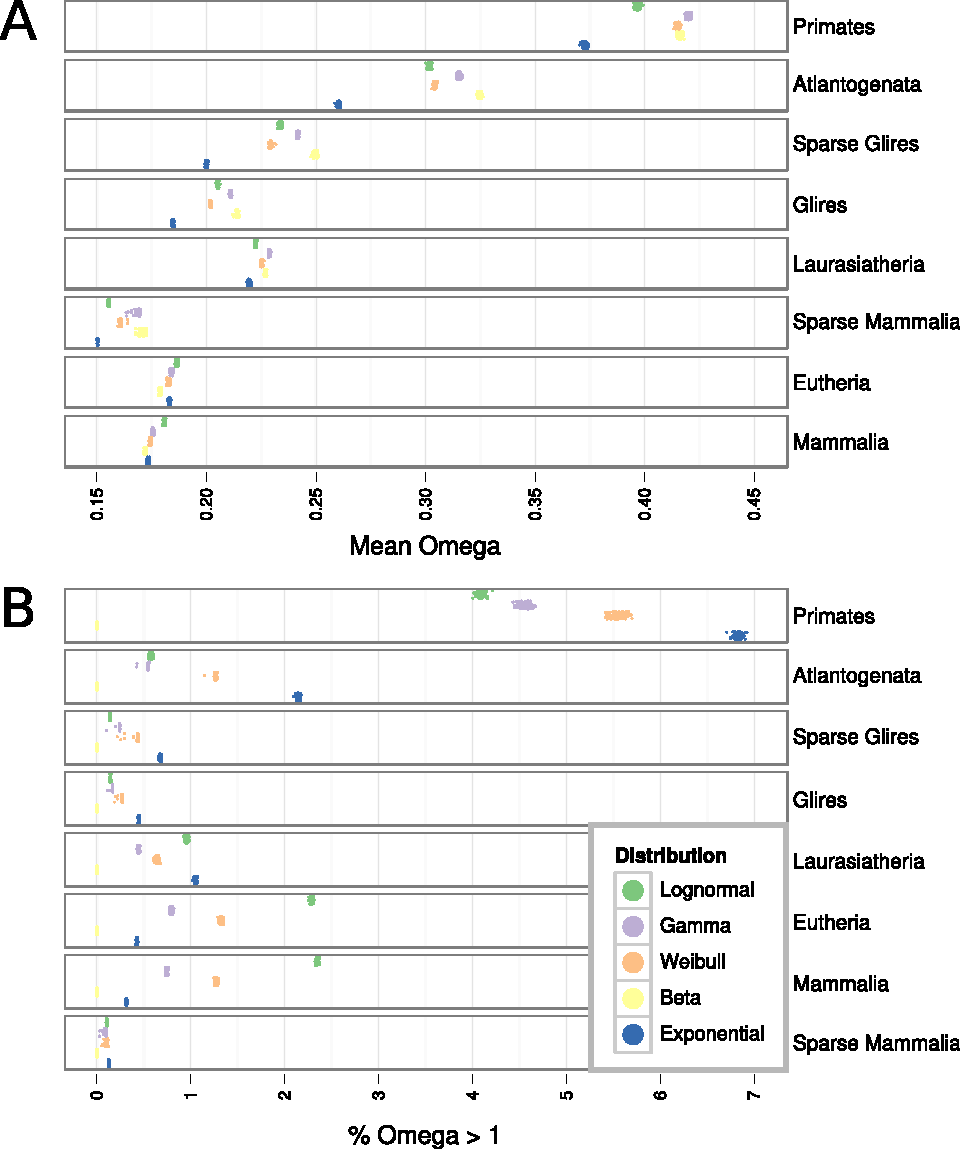
\includegraphics[scale=0.85]{Figs/distribution_fit_plots.pdf}
\caption{The mean value (A, Mean Omega) and the percentage of probability
  density with \omg$>1$ (B, Omega$>1$) from \ml fits of parametric distributions to
  sitewise \ci estimates. Each point represents the \ml fit of one
  distribution to 1 million points sampled from the genome-wide
  dataset with replacement; 100 such fits were generated for each
  distribution and species set. Note that the beta distribution is
  only defined on the interval (0,1), so the percentage of sites with
  \omg$>1$ was always zero.}
\label{fig_distribution_fit_plots}
\end{figure}

\draft{In preparation...}

\subsection{Evaluation of the effect of GC content and recombination rate on the \sw data}

\draft{In preparation...}

%\begin{figure}
%\centering
%\includegraphics[scale=0.85]{Figs/sorted_sites_gc.pdf}
%\caption{The effect of GC content on \sw estimates. Sitewise datasets
%  were filtered with the relaxed filter and sorted by the GC content
%  of the surrounding 100kb window. }
%\label{fig_sorted_sites_gc}
%\end{figure}


